\chapter{Experiments in neural reconstruction} \label{nerf_gsplat}

\section{Overview}

An additional objective we pursued to generate 3D photorealistic models of the robot's environment, leveraging images captured during the mapping process. Upon completion of mapping, our aim was to seamlessly integrate the robot's 3D model into this reconstructed scene. This integration would enable real-time simulation of the robot's movements during localization, transcending beyond a mere representation with a point cloud to deliver a highly realistic simulation experience.


\section{Using Spectacular AI to create input for NeRFs}

Continuing my exploration, I delved into the realm of 3D reconstruction using Neural Radiance Fields (NeRFs)~\cite{nerf}. To initiate this process, I utilized an example provided by the Spectacular AI SDK, specifically the \verb|mapping_visu.py| script. This script facilitated the creation of a mapping video, allowing for the specification of an output folder to store both the captured videos from the camera(s) and the resulting point cloud.

\begin{lstlisting}[language=bash,frame=single,float=!ht]
$ python3 mapping_visu.py --recordingFolder /PATH/TO/FOLDER
\end{lstlisting}

We have made significant progress, now possessing videos and a point cloud. However, these resources alone don't suffice as input for NeRFs, which demand a more specific format. NeRFs require not only the images captured at keyframes but also a COLMAP~\cite{colmap}, which contains essential information about the camera setup.

Keyframes serve as pivotal snapshots within the video sequence, capturing unique elements from various perspectives. These frames are crucial for determining the precise position and orientation of the camera at different points in the scene. Drawing a parallel from the animation realm~\cite{keyframes_in_animation}, keyframes are akin to markers that delineate significant moments or transitions between actions. In our context, these actions translate to movements such as forward progression or changes in direction.

Additionally, the COLMAP plays a pivotal role by providing foundational data about the camera configuration, including camera positions within each image and a point cloud derived from the scene mapping process. This comprehensive dataset serves as the backbone for NeRFs, enabling them to synthesize realistic renderings by leveraging both visual information and spatial context.

By integrating keyframes and COLMAP data, we can create a robust input pipeline for NeRFs, facilitating the generation of immersive and accurate 3D reconstructions from our captured videos and point cloud.

The long-discussed conversion can be done with the help of another Spectacular AI tool, called \verb|sai-cli|. It is a command line tool that can capture videos from OAK cameras and can execute the conversion for NeRF inputs. The required command for creating the input dataset for NeRFs is as follows:

\FloatBarrier
\begin{lstlisting}[language=bash,frame=single,float=!ht]
$ sai-cli process --format FORMAT --preview --preview3d INPUT OUTPUT
\end{lstlisting}

The execution of the command can be observed on Figure \ref{fig:sai_cli_process}. 

\begin{figure}[htbp]
	\centering
	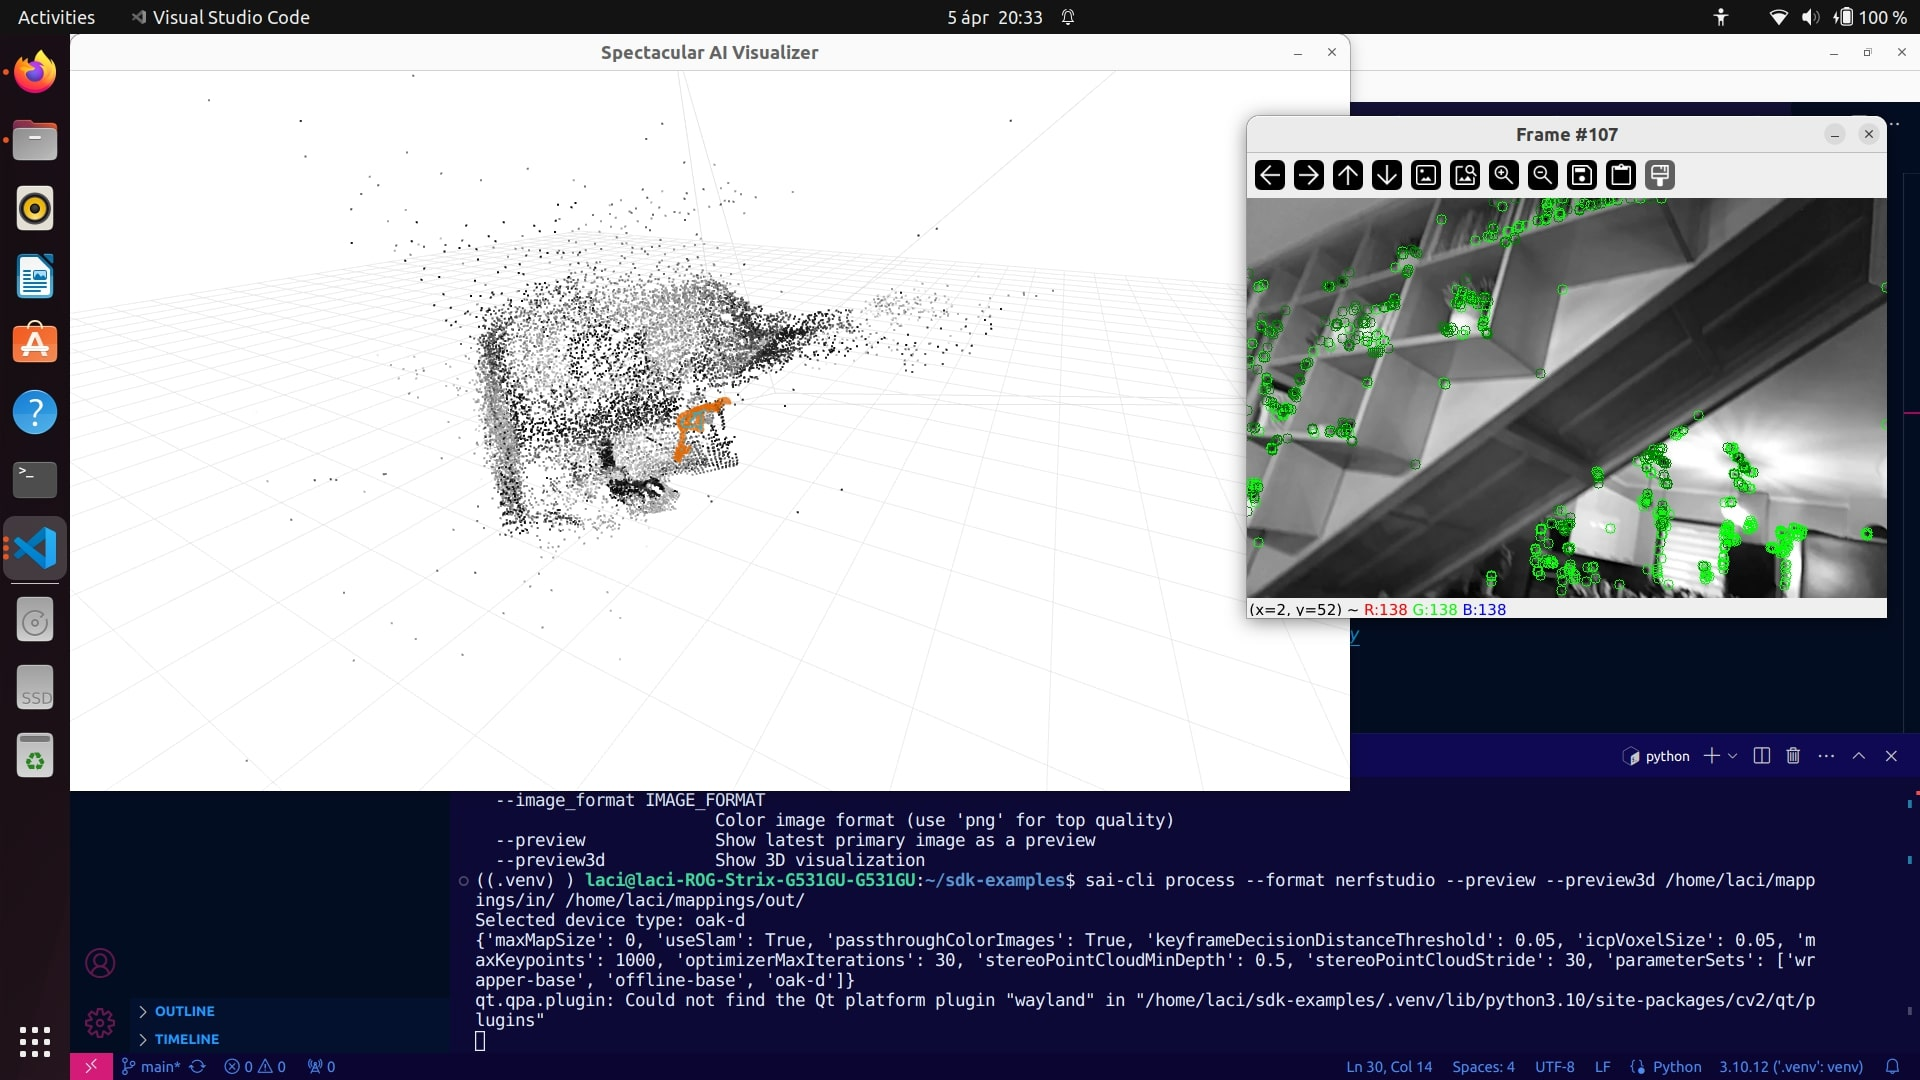
\includegraphics[width=150mm, keepaspectratio]{figures_jpg/sai-cli_process.jpg}
	\caption{Spectacular AI's CLI tool for creating input for NeRFs}
	\label{fig:sai_cli_process}
\end{figure}

\section{Experimenting with Nerfstudio}

With our input data ready, the next step for training a NeRF model was installing a suitable tool. For this, I chose to use Nerfstudio~\cite{nerfstudio}. However, frequent errors during installation with Conda prompted me to switch to a more straightforward solution: Docker\footnote{\url{https://www.docker.com/}}. While browsing DockerHub\footnote{\url{https://hub.docker.com/}}, I found that the official Docker image for Nerfstudio (nerfstudio/nerfstudio\footnote{\url{https://hub.docker.com/r/nerfstudio/nerfstudio}}) was poorly maintained: it was rarely updated, and it had only a single `latest` tag, making it impossible to pull previous versions. Fortunately, I discovered an alternative, well-maintained image (dromni/nerfstudio\footnote{\url{https://hub.docker.com/r/dromni/nerfstudio}}) that is frequently updated and includes a robust tagging system.

To start the Docker container with this image, I used the following command, which mounts the necessary input directories, grants GPU access, specifies the user, and increases shared memory for the container:

\FloatBarrier
\begin{lstlisting}[language=bash,frame=single,float=!ht]
$ sudo docker run --gpus all \
    -u $(id -u) \
    -v /home/laci/mappings/:/workspace/ \
    -v /home/laci/.cache/:/home/user/.cache \
    -p 7007:7007 --rm -it \
    --shm-size=1gb \
    dromni/nerfstudio:main
\end{lstlisting}

Once inside the container, training can be started with the following command:
\FloatBarrier
\begin{lstlisting}[language=bash,frame=single,float=!ht]
$ ns-train nerfacto --data PATH_TO_DATA
\end{lstlisting}

Nerfstudio offers a variety of NeRF models for training, but I followed the quickstart guide\footnote{\url{https://docs.nerf.studio/quickstart/first_nerf.html}} and chose the `nerfacto` model for simplicity. Figures \ref{fig:training_nerf_karcag} and \ref{fig:trained_nerf_karcag} show the training process and part of the trained model, respectively.

\begin{figure}[htbp]
	\centering
	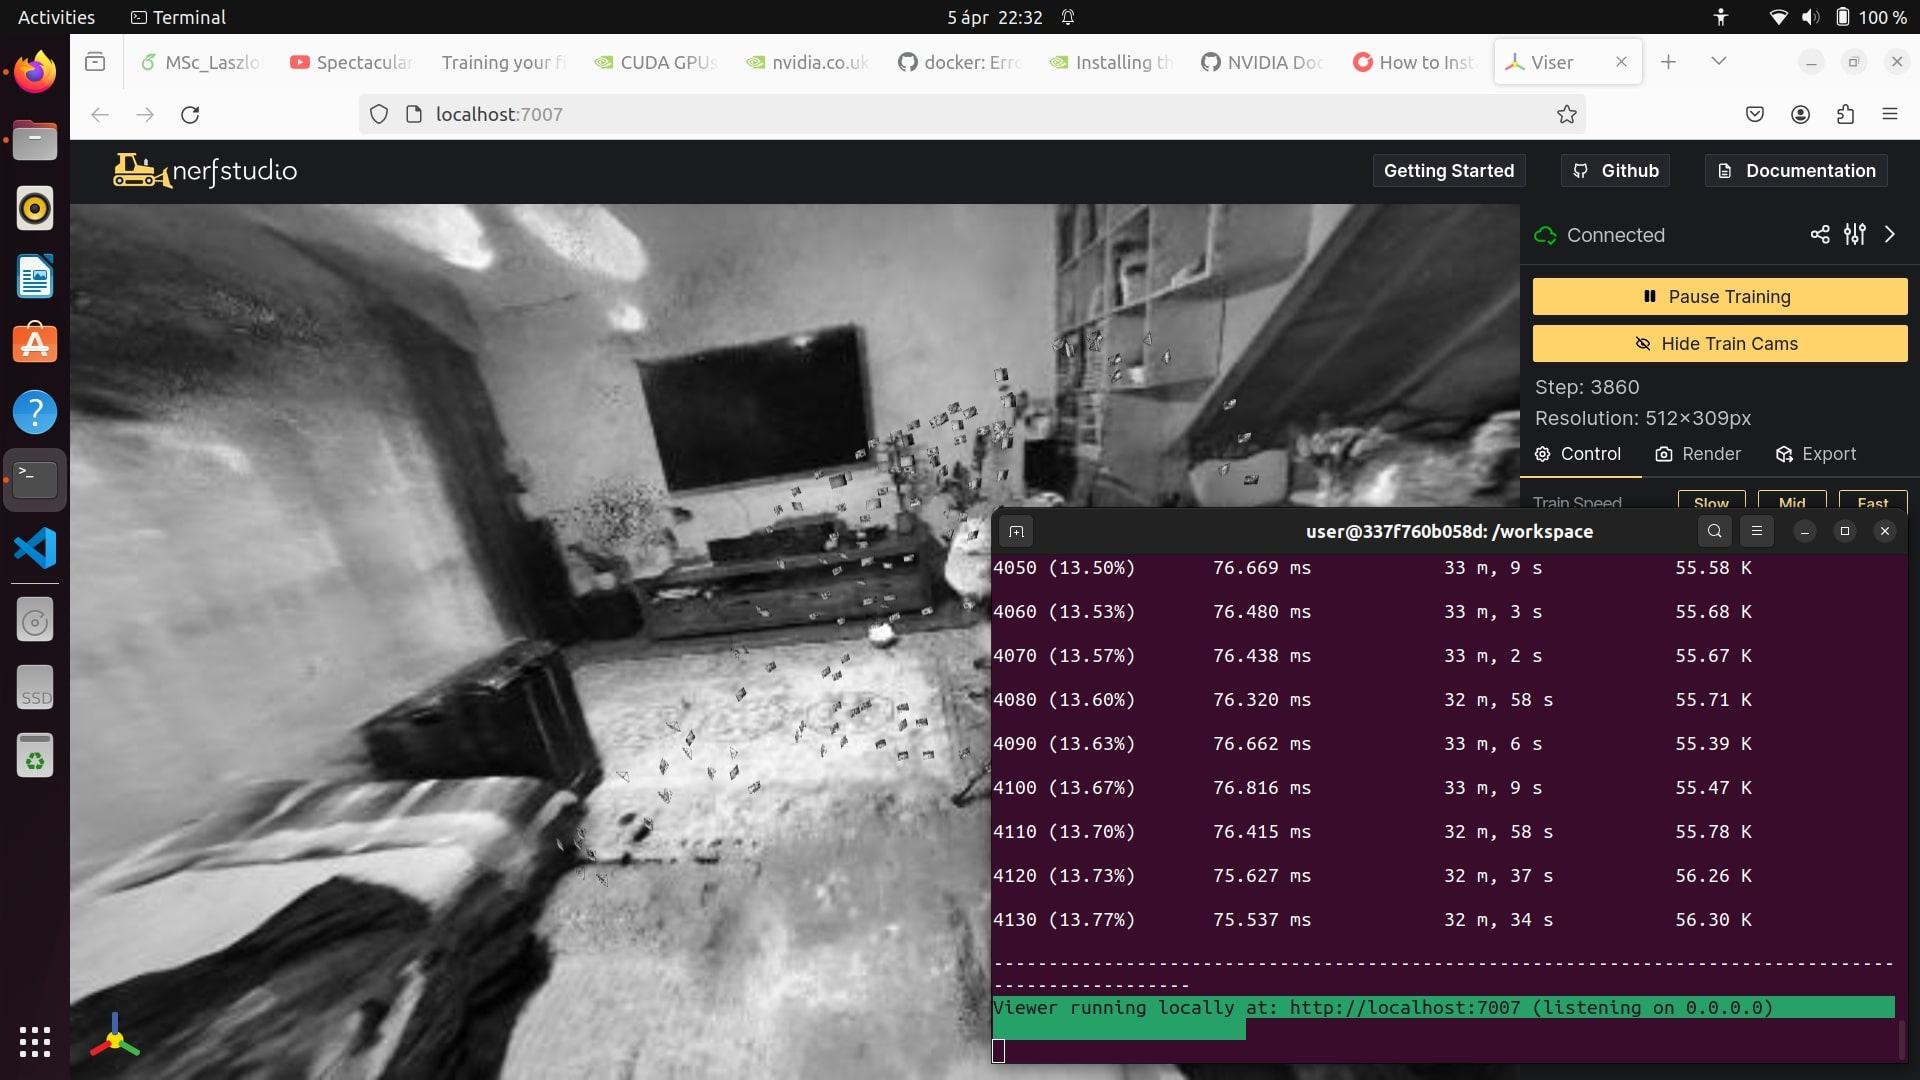
\includegraphics[width=150mm, keepaspectratio]{figures_jpg/nerfstudio.jpg}
	\caption{Training the nerfacto model}
	\label{fig:training_nerf_karcag}
\end{figure}

\begin{figure}[htbp]
	\centering
	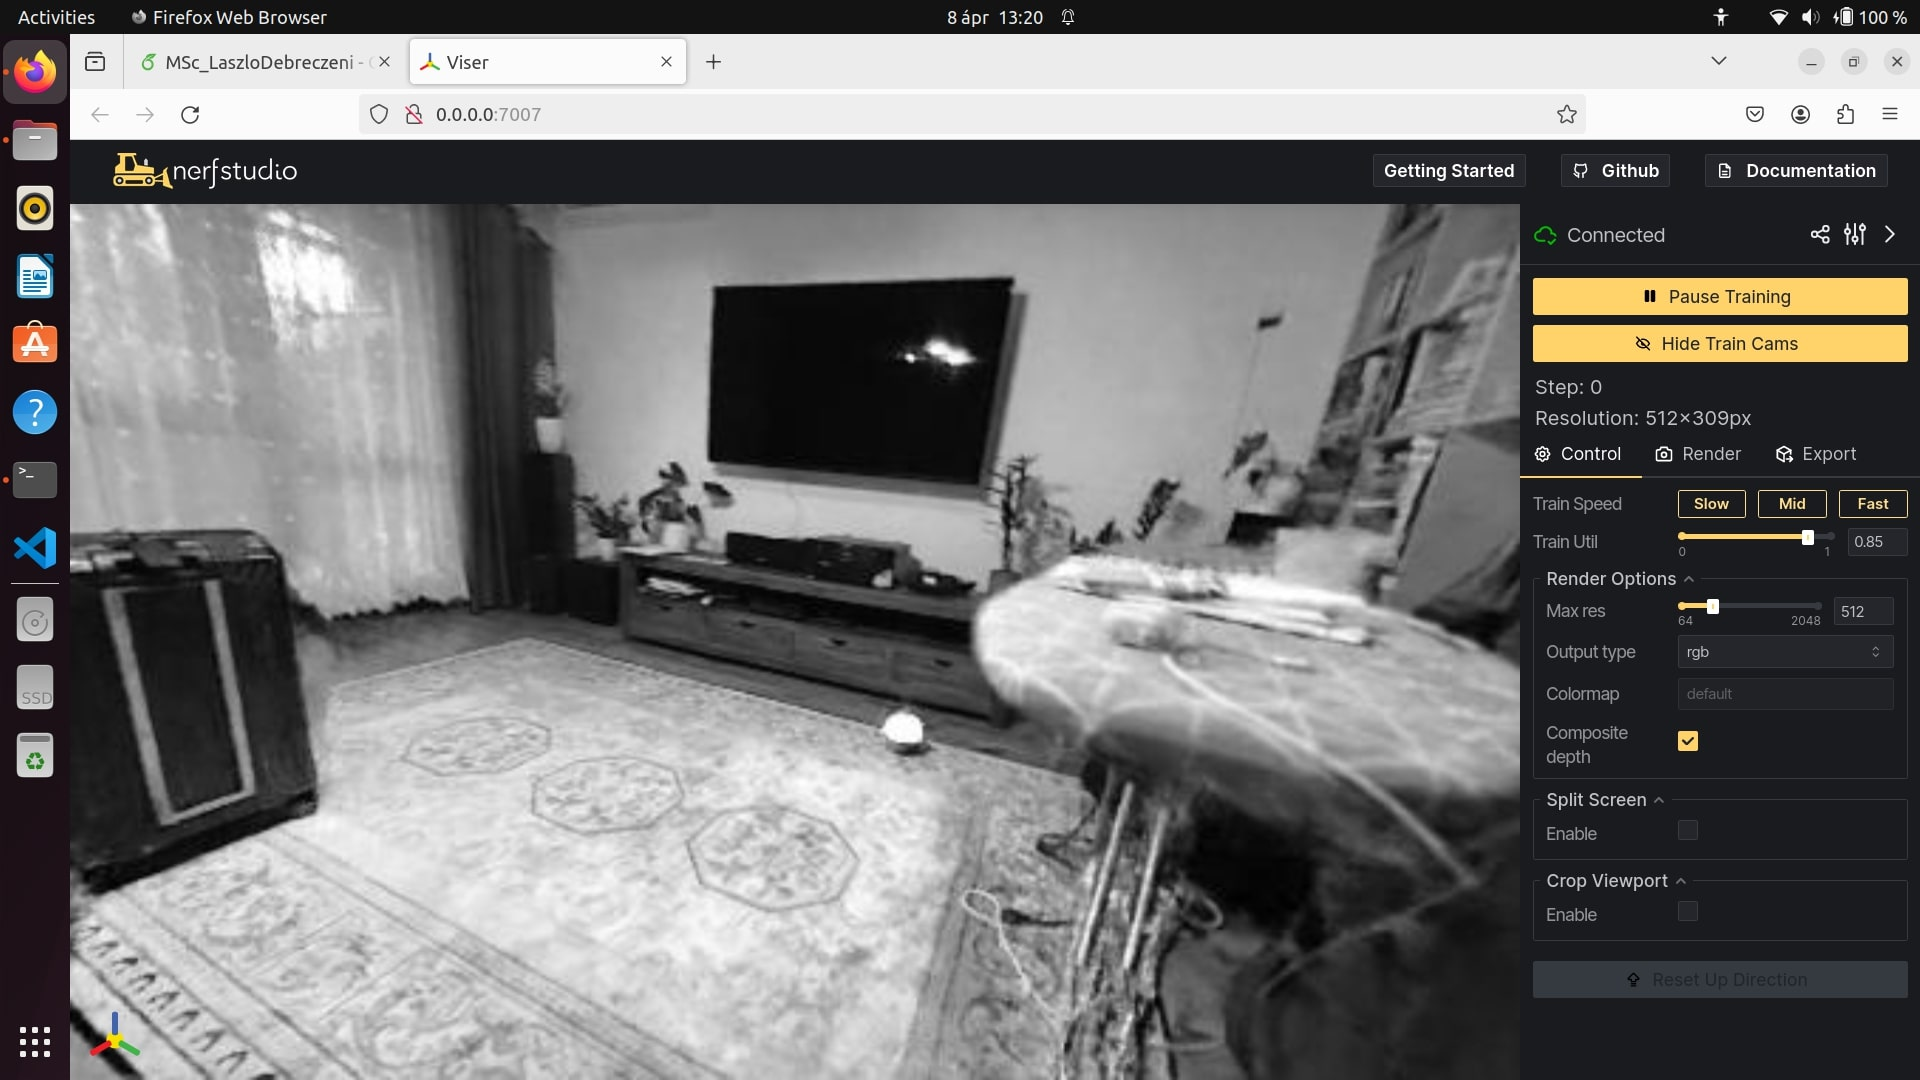
\includegraphics[width=150mm, keepaspectratio]{figures_jpg/trained_nerf_karcag1.jpg}
	\caption{Trained nerfacto model}
	\label{fig:trained_nerf_karcag}
\end{figure}

The results, while promising, were impacted by suboptimal input conditions. For instance, the video was captured in the late afternoon with artificial lighting, which led to reflections on the TV screen and other glossy surfaces, adding noise to the training process. Additionally, the USB3 cable for the camera—required for both power and data transmission—was relatively short, restricting my ability to capture all objects in the room from various angles. Consequently, certain areas of the scene appear blurry due to the lack of comprehensive coverage.

Nerfstudio also allows point cloud generation from the trained model. Users can specify parameters within the viewer, which generates a command for execution. A point cloud generated from the model is shown in Figure~\ref{fig:nerfstudio_point_cloud}.

\begin{figure}[htbp]
	\centering
	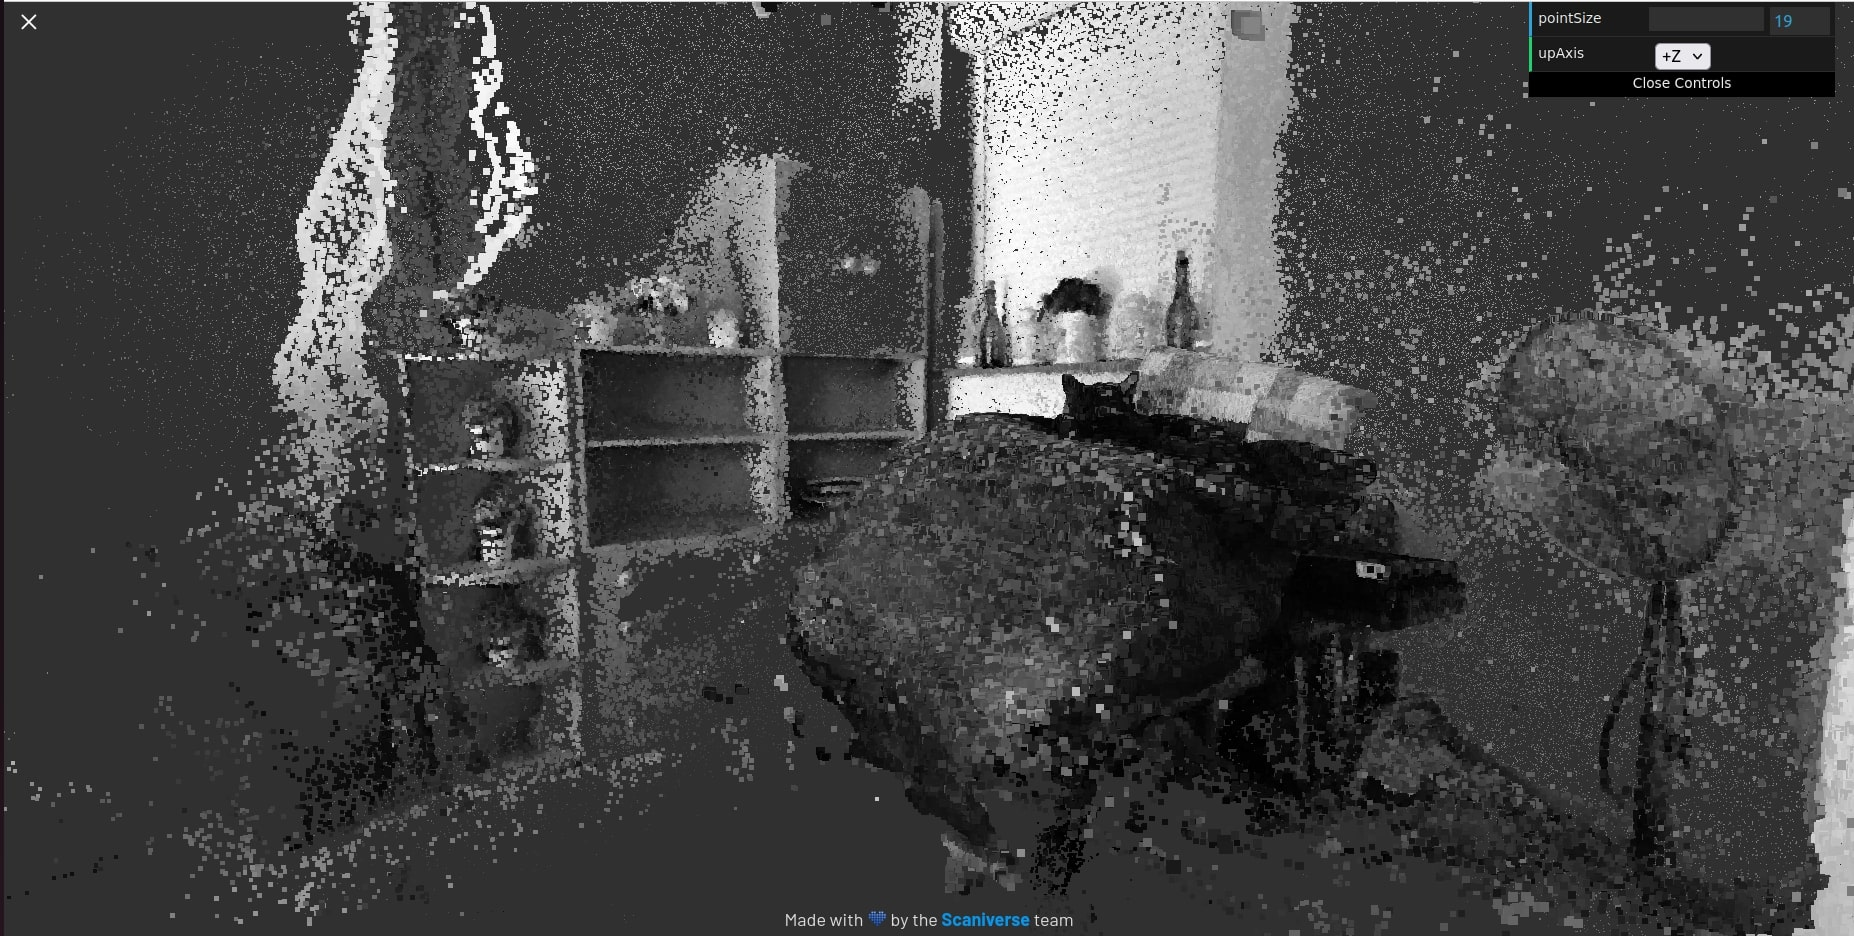
\includegraphics[width=150mm, keepaspectratio]{figures_jpg/nerfacto_point_cloud1.jpg}
	\caption{Point cloud from trained nerfacto model}
	\label{fig:nerfstudio_point_cloud}
\end{figure}

Despite these challenges, the final model was surprisingly accurate, validating the potential of NeRF technology. 

In a subsequent semester, I revisited Nerfstudio and attempted another installation via Conda, which, to my satisfaction, succeeded without errors. This allowed me to work natively on the system without Docker, streamlining my workflow significantly and eliminating the need for containerized setups.


\section{Experimenting with Luma AI}

In exploring NeRFs, we also experimented with Luma AI’s iOS application\footnote{\url{https://apps.apple.com/us/app/luma-ai/id1615849914}}, a more user-friendly approach to NeRF training (an Android version is available\footnote{\url{https://play.google.com/store/apps/details?id=ai.lumalabs.polar&hl=en_US&pli=1}} too). This app requires a LiDAR-equipped phone; I used an iPhone 13 Pro, and the app performed flawlessly on it. I selected my cat Szotyi’s toy for testing, first defining the object’s dimensions in an AR view, then capturing images from various angles. The app automatically uploaded these to the cloud, where it trained a NeRF. Once complete, the NeRF was remarkably lifelike, as if the toy were right in front of me, as shown in Figure~\ref{fig:luma_ai_szotyi_toy}.

\begin{figure}[htbp]
	\centering
	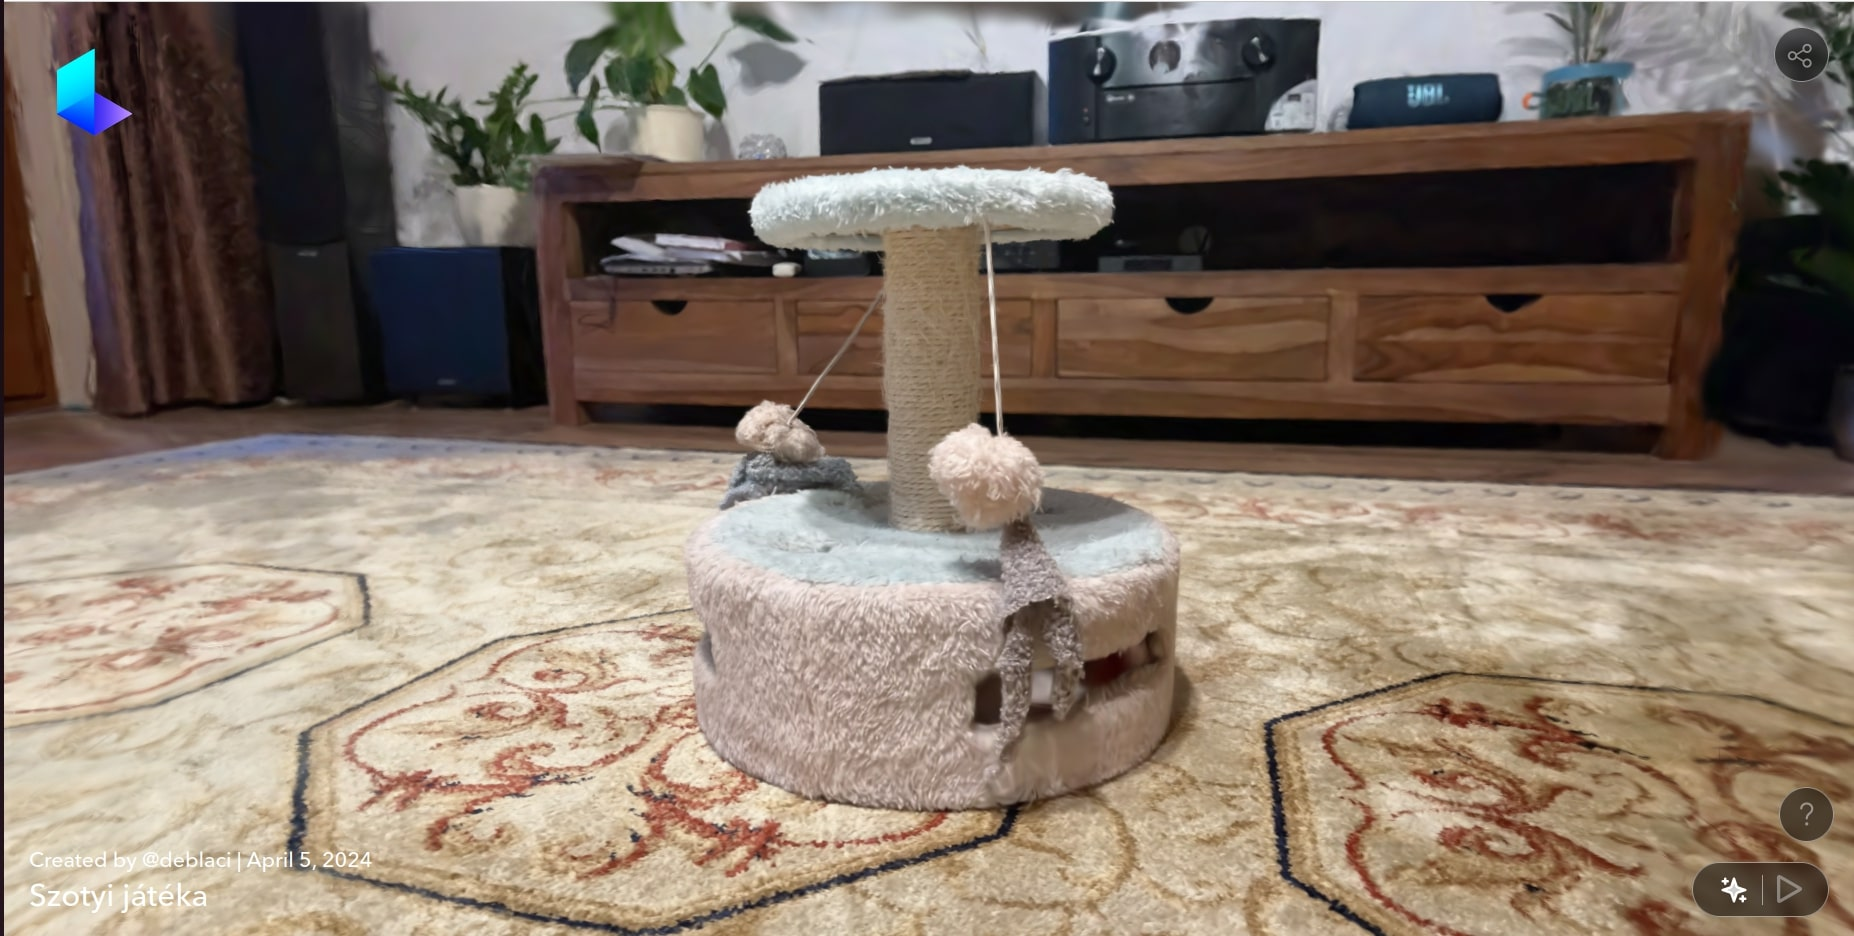
\includegraphics[width=150mm, keepaspectratio]{figures_jpg/szotyi_jateka_luma_ai.jpg}
	\caption{Szotyi's toy recreated by Luma AI}
	\label{fig:luma_ai_szotyi_toy}
\end{figure}

\section{Experimenting with Gaussian Splatting}

To further explore photorealistic reconstructions, we experimented with Gaussian Splatting~\cite{3DGS}. Since Nerfstudio offers a model utilizing Gaussian Splatting, called \texttt{splatfacto}~\cite{splatfacto}, I chose to work with this model due to my existing experience with Nerfstudio. However, using the \texttt{dromni/nerfstudio} Docker image caused persistent CUDA errors as it failed to detect the installation, despite its presence. After hours of troubleshooting, I switched to the official \texttt{nerfstudio/nerfstudio} image, only to encounter a different error:

\FloatBarrier
\begin{lstlisting}[language=bash,frame=single,float=!ht]
assert block width > 1 and block width <= 16, 
"block width must be between 2 and 16"
AssertionError: block width must be between 2 and 16
\end{lstlisting}

Investigation revealed that this issue stemmed from low-level incompatibilities within either Nerfstudio or the \texttt{splatfacto} model\footnote{\url{https://github.com/nerfstudio-project/gsplat/issues/159}}. Upgrading the \texttt{gsplat} package proved ineffective.

In response, I tried an alternative Gaussian Splatting implementation\footnote{\url{https://github.com/graphdeco-inria/gaussian-splatting}}, which successfully began training but consistently failed with \texttt{CUDA out of memory} errors. This implementation demands 24 GB of VRAM, exceeding my GTX 1660’s 6 GB capacity. Using Google Colab as an alternative initially worked but ultimately failed due to memory limitations during the saving process. Fortunately, my advisor Gábor was able to complete training on his GTX 1080 GPU, though the result was disappointingly blurry.

In my second semester, Gaussian Splats again became essential, particularly for representing the robot’s mapped environment. I revisited \texttt{nerfstudio}'s \texttt{splatfacto} and \texttt{splatfacto-big} models, which had been updated since my previous attempts. This time, the models successfully ran on my GTX 1660 GPU, eliminating the need for external support. An example Gaussian Splat I generated is shown in Figure~\ref{fig:spai_gsplat}.
